% !TeX document-id = {be34c84b-deee-4ae7-a020-3510ae5ecf87}
%%% File encoding: UTF-8
%%% äöüÄÖÜß  <-- keine deutschen Umlaute hier? UTF-faehigen Editor verwenden!

%%% Magic Comments zum Setzen der korrekten Parameter in kompatiblen IDEs
% !TeX encoding = utf8
% !TeX program = pdflatex 
% !TeX spellcheck = de_DE
% !BIB program = biber

\documentclass[bachelor,german]{hgbthesis}
% Zulässige Optionen in [..]: 
%   Typ der Arbeit: diploma, master (default), bachelor, internship 
%   Hauptsprache: german (default), english
%%%----------------------------------------------------------

\RequirePackage[utf8]{inputenc}		% bei der Verw. von lualatex oder xelatex entfernen!

\graphicspath{{images/}}    % Verzeichnis mit Bildern und Grafiken
\logofile{}				% Logo-Datei = images/logo.pdf (\logofile{}, wenn kein Logo gewünscht)
\bibliography{references}  	% Biblatex-Literaturdatei (references.bib)

%%%----------------------------------------------------------
\begin{document}
%%%----------------------------------------------------------

\begin{center}
	\begin{Huge}
	Erweiterungsentwicklung für Microsoft Dynamics 365 Business Central unter Verwendung von ExtensionsV2
	\end{Huge}

	\begin{Large}
	\bigbreak
	Johannes Naderer
	
	(se0307)
	\end{Large}	
\end{center}
\begin{center}
	
\end{center}
%%%----------------------------------------------------------
\frontmatter                    % Titelei (röm. Seitenzahlen)
%%%----------------------------------------------------------

%\maketitle
\tableofcontents

%%%----------------------------------------------------------
\mainmatter          % Hauptteil (ab hier arab. Seitenzahlen)
%%%----------------------------------------------------------

\chapter{Kurzfassung}
\label{cha:Kurzfassung}
Cloud Computing bietet Software Herstellern bisher nicht vorhandene technische Möglichkeiten zur Erstellung von hoch skalierbaren Hardware Infrastrukturen. Um diese Möglichkeiten mit der bestehenden Software \textit{Microsoft Dynamics 365 Business Central} zu nutzen, und gleichzeitig die Vorteile des Systems zu wahren, wurde ein neues Programmierkonzept eingeführt. Code-Änderungen, wie sie bisher die Norm waren, sind in einem Cloud-System nicht akzeptabel. Daher wurde das Konzept der erweiterungsbasierten Programmierung mit ExtensionsV2 eingeführt. ExtensionsV2 erlaubt es Entwicklern, die Grundfunktionalität des ERP-Systems zu erweitern, ohne die Stabilität und Updatefähigkeit des Systems negativ zu beeinflussen.


Diese Arbeit vermittelt einen Überblick über das Programmsystem \textit{Microsoft Dynamics 365 Business Central}, der verwendeten Schichtenarchitektur und vergleicht die Programmierkonzepte hinter den beiden Sprachen C/AL und AL.


Nach der Definition des Begriffs \textit{ERP-System} und der geschichtlichen Entwicklung des Systems \textit{Microsoft Dynamics 365 Business Central} werden die verschiedenen Arten von Objekten, die als Grundbausteine des Systems fungieren beleuchtet. Im Hauptteil wird das neue Programmiermodell mit ExtensionsV2 mit der Code-Anpassung unter C/AL verglichen.  Um einen quantifizierbaren Vergleich zu ermöglichen wird eine Erweiterung für das System mit beiden Arten der Programmierung umgesetzt. Da beide Implementierungen schlussendlich dieselbe Funktionalität zur Verfügung stellen, kann so speziell auf die Unterschiede zwischen den beiden Programmierparadigmen eingegangen werden. Anschließend werden Laufzeitmessungen durchgeführt, um Differenzen zwischen den Implementierungen aufzudecken. Abschließend werden die Implikationen bezüglich zeitgemäßer Entwicklungswerkzeuge wie Source Code Management und CI/CD diskutiert, die mit dem dateibasierten Entwicklungsprozess in der erweiterungsbasierten Programmierung in Visual Studio Code und AL einher gehen.
\chapter{Abstract}
\label{cha:Abstract}

Cloud computing offers software manufacturers previously unavailable technical possibilities for creating highly scalable hardware infrastructures. To take advantage of these capabilities with the existing software \textit{Microsoft Dynamics 365 Business Central} while maintaining the benefits of the system, a new programming concept has been introduced. Code changes, as previously the norm, are unacceptable in a cloud system. Therefore, the concept of extension-based programming with ExtensionsV2 has been introduced. ExtensionsV2 allows developers to extend the basic functionality of the ERP system without negatively affecting the stability and updating capability of the system.


This thesis provides an overview of the program system \textit {Microsoft Dynamics 365 Business Central}, the used layer architecture and compares the programming concepts behind the two languages C/AL and AL).


Following the definition of the term \textit{ERP system} and the historical development of the system \textit{Microsoft Dynamics 365 Business Central}, the various types of objects that function as the basic building blocks of the system are examined. The main part compares the new programming model with ExtensionsV2 with the code adaptation with C/AL. To allow a quantifiable comparison, an extension for the system is implemented with both types of programming. Since both implementations ultimately provide the same functionality, it is possible to specifically address the differences between the two programming paradigms. Next, runtime measurements are performed to reveal differences between the implementations. Finally, the implications of contemporary development tools such as source code management and CI/CD are discussed, which go hand in hand with the new file-based development process in extension-based programming in Visual Studio Code and AL.
\chapter{Einleitung}
\label{cha:Einleitung}

\section{Motivation}
\label{sec:Motivation}

ERP-Systeme sind heute aus dem wirtschaftlichen Umfeld nicht mehr wegzudenken \cite{WongTein2003} \cite{DuplagaMarzie2003}. Bereits in den 1970er Jahren erkannten Wirtschaftstreibende Potential darin, ihre Prozesse und Unternehmensdaten zu digitalisieren. Während in den 1970er und 1980er Jahren innerhalb der einzelnen Abteilungen eines Unternehmens verschiedene Softwarelösungen zum Einsatz kamen, ist man sich mittlerweile einig, dass eine zentrale Applikation zur Verwaltung aller unternehmerisch wichtigen Daten und Prozessschritte große Vorteile liefert. Diese Erkenntnis hatte zur Folge, dass kleine Softwarehersteller immer mehr ins Wanken gerieten, da von der Wirtschaft allumfassende Software-Giganten gefordert wurden, die eine Vielzahl von Anforderungen aus den verschiedensten Anwendungsdomänen zu erfüllen hatten. Solche Systeme können mit den meist begrenzten Ressourcen kleiner und mittelständischer Hersteller erfahrungsgemäß nicht im geforderten Umfang entwickelt werden. Gleichzeitig entstanden durch die gewachsenen Anforderungen umfassende Softwaresysteme einiger größerer Hersteller, hier sind vor allem Marktführer SAP, aber auch Microsoft mit seiner Dynamics Sparte zu nennen.

Wer heute in einem Unternehmen mit der Einführung eines ERP-Systems betraut wird, muss sich intensiv mit den verschiedenen erhältlichen Lösungen auseinander setzen\cite{WongTein2003}. Denn neben Lizenzierung und finanziellen Aspekten, ist auch zu erarbeiten, welche Systeme die bestehenden Prozesse des Unternehmens am Besten abbilden. Systeme bilden Geschäftsprozess meist auf eine bestimmte Art ab. Sollte diese nicht mit dem Vorgehen des Unternehmens überein stimmen, bleibt meist nur einer von zwei möglichen Auswegen offen. Entweder das Unternehmen passt seine Prozesse an die Vorgabe des Systems an, oder das System muss entsprechend angepasst werden, um den Ansprüchen des Unternehmensprozesses zu genügen.

Und genau hier spielt die Anpassbarkeit und Erweiterbarkeit eines Systems die zentrale Rolle. Gerade branchenspezifische und insbesondere unternehmensspezifische Prozesse müssen meist erst programmiert und in das System integriert werden. Programmierarbeiten und Änderungen an den standardmäßigen Prozessen sind meist aufwendig, und stellen so ein nicht zu vernachlässigendes finanzielles Risiko dar.

Um die Aspekte der Erweiterbarkeit und Anpassungsmöglichkeit möglichst gut zu erfüllen, entschied sich Microsoft im ERP-System \textit{Microsoft Dynamics NAV} bereits in sehr frühen Versionen dazu, zertifizierten Entwicklern freien Zugang zum Applikationscode zu gewähren\cite{BrummelPatterns2015}. So können Entwickler die gesamte Geschäftslogik des Systems je nach Unternehmensanforderungen nach Belieben abändern und erweitern, in dem sie neuen Programmcode hinzufügen, oder den Standardcode von Microsoft anpassen oder gegebenenfalls auch löschen. Dies hat zum Einen zur Folge, dass Entwickler mächtige Applikationen erstellen können und sich diese direkt in das bestehende System integrieren lassen. Allerdings kommen mit diesen umfassenden Möglichkeiten auch Probleme auf. Je weiter die oft über Jahrzehnte verwendeten und erweiterten Systeme von Microsofts Codebasis abweichen, desto aufwendiger, fehleranfälliger und teurer ist es, diese Systeme mit den Aktualisierungen des Herstellers zu versorgen, die periodisch in das System integriert werden müssen.  

Um die Systeme updatefähig zu halten, und gleichzeitig ein Entwicklungsmodell zu schaffen, dass auch in der Cloud-Variante des ERP-Systems funktionieren kann, wurde mit Dynamics NAV 2017 erstmals das Konzept der Erweiterungsprogrammierung mit ExtensionsV1 für Dynamics NAV vorgestellt. ExtensionsV1 ist ein gänzlich neuer Ansatz für das ERP-System zu programmieren und hat konzeptionell viele Vorteile gegenüber der konventionellen Art zu entwickeln, ist aber mittlerweile aufgrund einiger technischer Schwierigkeiten obsolet.

Mit der in 2018 veröffentlichten Version - ExtensionsV2 - sind nicht nur viele der technischen Mängel behoben, ExtensionsV2 kommt auch mit einer neuen Programmiersprache und Entwicklungsumgebung.

\section{Zielsetzung}
\label{sec:Zielsetzung}
Im Rahmen dieser Arbeit wird ein Überblick über die ERP-Plattform, die sich mittlerweile \textit{Microsoft Dynamics 365 Business Central} nennt, und die Programmierung dieses Systems gegeben. Hierfür wird erst eine Übersicht über das Gesamtsystem und seine Schichtenarchitektur vermittelt. Anschließend wird das Konzept der Erweiterungsentwicklung mit ExtensionsV2 mit der konventionellen prozeduralen Entwicklung verglichen. Dies erfolgt anhand eines Beispiels, das auf beide Arten gelöst wird. Einerseits wird die Anwendung in der Entwicklungsumgebung C/SIDE mit C/AL entwickelt. Andererseits wird anhand der Aufgabenstellung eine Erweiterung mit ExtensionV2 in Visual Studio Code und der aktuellen Sprache AL erstellt. Hierbei liegt der Fokus nicht darauf, kleine syntaktischen Unterschiede zwischen den Sprachen hervorzuheben, sondern Neuerungen in der Sprache AL zu beleuchten, und konzeptionelle Unterschiede zwischen den beiden Programmierparadigmen aufzuzeigen und zu bewerten.

Der Vergleich erfolgt primär anhand von Laufzeitmessungen. Zusätzlich wird auch diskutiert, welche Vor- und Nachteile sich durch die nun neue dateibasierte Codeverwaltung hinsichtlich der Einbindung und Nutzung von Source Code Management und Continuous Integration Systemen ergeben. In einem letzten Block wird danach das Event-basierte Programmiermodell der Erweiterungsentwicklung mit ExtensionsV2 diskutiert, die Vor- und Nachteile beleuchtet, die mit dem Wechsel von Code-Anpassung hin zu Code-Erweiterung einher gehen.


\chapter{Stand der Technik}
\label{cha:Stand der Technik}

\section{ERP: Definition und Übersicht}
\label{sec:ERP: Definition und Übersicht}
ERP Systeme sind umfangreiche kommerzielle Softwaresysteme, mit der Kernaufgabe, alle Abteilungen und Prozesse eines Unternehmens soweit wie möglich digital abzubilden\cite{doi:10.1002/smr.239}. Ein ERP-System stellt für ein Unternehmen somit eine zentrale Verarbeitungs- und Datensicherungsplattform für sämtliche unternehmensrelevanten Geschäftsdaten bereit. Die Daten sind hierbei in einem einzelnem System erfasst, und sind so sofort für alle Unternehmensbereiche verfügbar. Es sind keine Synchronisierungsschritte oder Schnittstellen innerhalb des Systems nötig. Durch die zentrale Datenerfassung, stellt ein ERP-System eine durchgängige Informationsquelle für alle Unternehmensbereiche dar, die bei der Prozessanalyse und Analyse als Datenbasis für geschäftliche Entscheidungsträger unabdingbar ist.

Im Gegensatz zu abteilungsbezogenen Systemstrukturen (Insellösungen) ist es durch Einsatz eines ERP-Systems möglich Funktionen zu nutzen, für deren Durchführung Informationen aus mehreren Abteilungen nötig sind\cite{DynamicsNAV2018Anwenderbuch}. So kann zum Beispiel bei Eingang eines Auftrags sofort automatisiert geprüft werden, ob der Auftrag angenommen werden soll. Entscheidungen wie diese basieren auf einem sehr breiten Datenstamm aus den verschiedenen Abteilungen. Aus den Daten der Finanzabteilung können Zahlungsmoral, offene Beträge des Kunden und ein voraussichtlicher Deckungsbeitrag eine Rolle für diese Entscheidung spielen. Anhand der Lagerhaltungsdaten kann sofort eine Verfügbarkeitsprüfung für die bestellten Artikel durchgeführt werden. Mithilfe von Produktions- und Personaldaten wird ausgewertet, ob ausreichend Personal und Maschinenressourcen für die Erfüllung des Auftrags zur Verfügung stehen. Dies sind nur einige wenige Beispiele, wie ein ERP-System bei der täglichen unternehmerischen Tätigkeit behilflich sein kann.

Da in ERP-Systemen der Zugriff auf die Datenbank nicht durch die Systemarchitektur eingeschränkt ist, muss der Zugang zu den Daten im System über ein Rechte- und Modulsystem gesteuert werden\cite{DynamicsNAV2018Anwenderbuch}. Berechtigungssätze lassen sich hier meist sehr feingranular definieren, sodass einerseits der Schutz sensibler Daten gewährleistet ist, jedoch andererseits alle benötigten Daten entsprechend betrachtet und verarbeitet werden können.

\pagebreak

\begin{figure}[h]
	\centering
	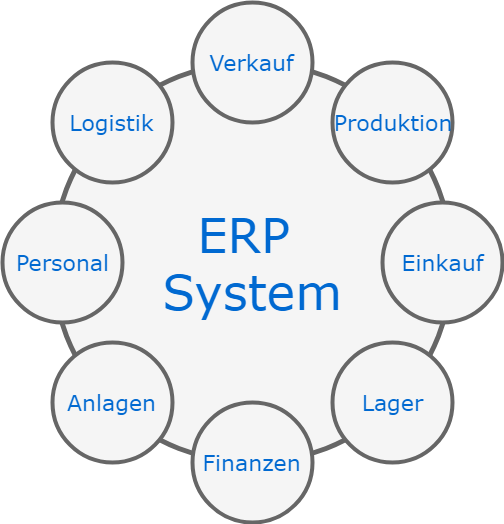
\includegraphics[width=70mm]{images/ERPModules.png}
	\caption{Schematische Darstellung: Modularisierung anhand Unternehmensabteilung}
	\label{fig:Modulisierung}
\end{figure}

Um die umfangreichen Funktionalitäten eines ERP-Systems zu gliedern und aufzuteilen, bedienen sich die meisten Hersteller eines Modul-Systems. Meist spiegelt die Aufteilung dieser Module die einzelnen Abteilungen eines Unternehmens wieder. So verteilt sich die Gesamtfunktionalität eines Systems beispielsweise auf ein Einkaufsmodul, ein Vertriebsmodul und viele andere Teilbereichsmodule auf. 
Diese Module können in ihren Grundzügen unabhängig voneinander verwendet werden. So kann ein Unternehmen beispielsweise entscheiden, vorerst nur Finanzen und Personal über das System zu verwalten. Andere Module können im Laufe der Zeit stückweise in Betrieb genommen werden. Zu den bekanntesten ERP Herstellern zählen unter anderen IBM, SAP, Microsoft, Infor und Sage.

\pagebreak
\section{Geschichte und Grundarchitektur Dynamics 365 Business Central}
\label{sec:Grundarchitektur Dynamics 365 Business Central}

\subsection{Geschichte}
\label{subsec:Geschichte}
Das ERP-System, dass heute \textit{Microsoft Dynamics 365 Business Central} heißt, erschien ursprünglich 1984 unter dem Namen \textit{PCPlus} als ein ERP System für Microsoft DOS in Dänemark\cite{DesignAndImplementationGayer}. Während seiner mittlerweile 35-jährigen Geschichte wurde das Produkt einige Male neu benannt und an den technischen Fortschritt angepasst. Was 1984 begann, wurde 1995 unter dem Namen \textit{Navision Financials} als das erste ERP-Produkt mit grafischer Benutzeroberfläche für Windows95 präsentiert. 2002 wurde \textit{Navision Financials} von Microsoft gekauft und unter dem Namen \textit{Microsoft Business Solutions Navision} vertrieben. In all diesen Jahren basierte die Datenspeicherung des Systems in einem komplexen Dateibasierten Format. Im Jahr 2008 passiert dann der Schritt zu Microsoft SQL Server und der 3-Schichten-Architektur, nun unter dem Namen \textit{Microsoft Dynamics NAV 2009}. Der vorerst letzte Meilenstein in der Geschichte des Systems ist 2018. Das System wird nun als Cloud-ERP-System unter dem Namen \textit{Microsoft Dynamics 365 Business Central} betrieben.

Trotz den vielen Versionen und der jahrzehntelangen Geschichte dieses Systems, finden sich auch in der heutigen Code-Basis noch viele Passagen, die bereits in den 1980er Jahren entstanden, und bis heute produktiv eingesetzt werden.

\subsection{3-Schichten Architektur}
\label{subsec:3-Schichten Architektur}
Dynamics 365 Business Central basiert auf einer 3-Schichten Architektur. Durch Schichtenarchitekturen lassen sich die Aufgabengebiete bzw. Teile eines komplexen Softwaresystems aufteilen. Im Falle von Dynamics Business Central 365 unterscheiden wir zwischen der Endbenutzerschicht, der Serverschicht und der Datenbankschicht.

\begin{figure}[h]
	\centering
	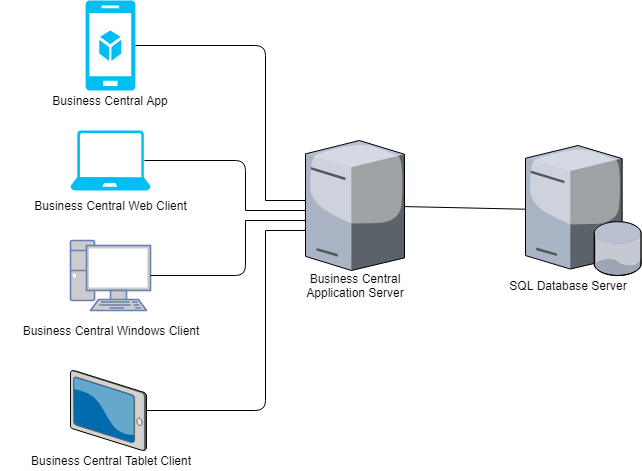
\includegraphics[width=100mm]{images/3TierArchitecture.png}
	\caption{Dynamics 365 Business Central: 3-Schichten Architektur}
	\label{fig:Image3TierArchitecture}
\end{figure}

\pagebreak

Schicht 1: Die Endbenutzerschicht/Präsentationsschicht: 
In dieser Schicht der Architektur finden sich sämtliche Softwarekomponenten, die direkt die von der Serverschicht exportierten Funktionalitäten nutzen. Hierzu zählen vorrangig die von Microsoft veröffentlichten Endbenutzerprogramme wie der Business Central WebClient und die Business Central Mobile App. Aber auch von Drittanbietern erstellte Softwarekomponenten, die Microsoft Graph API oder von Business Central veröffentlichte Webdienste nutzen sind Teil der Endbenutzerschicht.
\linebreak

Schicht 2: Die Serverschicht: 
Die Business Central Serverapplikation (auch \textit{Middle-Tier} oder \textit{Service-Tier}) stellt das Herzstück des Gesamtsystems dar. Der Business Central Server ist eine .NET basierte Serveranwendung und nutzt die Windows Communication Foundation (WCF) als Kommunikationsprotokoll. Der Server nimmt sämtliche Anfragen von Endbenutzerprogrammen entgegen, holt anhand dieser Anfragen Daten von der Datenbankschicht ab, führt mithilfe der abgeholten Daten Geschäftslogik aus, bereitet die Ergebnisse der Geschäftslogik auf, und liefert diese zurück an das anfragende Endbenutzerprogramm. Neben den Endpunkten zur Client-Kommunikation beinhaltet die Serverkomponente auch die Webserverkomponenten zur Nutzung des WebClients. Die Webserverkomponente selbst ist eine ASP.NET Core Applikation, die auf einem mitgeliefertem IIS (Internet Information Server) läuft. Daher ergibt sich auch die Anforderung, dass die Serverschicht auf einer Windows-Server Maschine betrieben werden muss.
\linebreak

Schicht 3: Die Datenbankschicht:
Hinter der Datenbankschicht verbirgt sich eine Microsoft SQL Server Instanz. Hierbei ist zu erwähnen, dass aufgrund der historischen Entwicklung des Gesamtsystems einige Funktionen einer klassischen relationalen Datenbank hier nicht verwendet werden. So wird man am Datenbankserver vergeblich nach Relationen zwischen Tabellen suchen (Fremdschlüsselbeziehung), denn diese existieren hier schlichtweg nicht. Diese Beziehungen werden von der Serverschicht verwaltet. Auf Grund dieser Tatsache ist es strengstens abzuraten manuell mit SQL Befehlen Datenbestände zu ändern. Änderungen, die nicht durch die Logik der Serverschicht validiert werden können, können schnell zu Inkonsistenzen in den Daten führen, die in weiterer Folge das Gesamtsystem korrumpieren und zu Systemausfällen führen können. 
\linebreak

Die Unterteilung der einzelnen Teilbereiche des Systems in drei Teilbereiche liefert einige Vorteile. So können anhand der vom Server exportierten Schnittstellen schnell neue Apps und 



\pagebreak
\section{Objektarten in Business Central}
\label{sec:Objektarten in Business Central}
\chapter{Vergleich}
\label{cha:Vergleich}
\chapter{Tests und Evaluierung}
\label{cha:Tests und Evaluierung}

\section{.NET Klassenbibliothek und AL-Sprachkonstrukte}
\subsection{Testaufbau}
Im ersten Testaufbau werden die im Treuepunkt-Beispiel \ref{sec:Aufgabenstellung} verwendeten Varianten der Webservice Kommunikation gemessen und auf ihr Laufzeitverhalten untersucht. In diesem Test werden beide Varianten eine große Anzahl von Http-Anfragen erstellen und an einen Webdienst übermitteln. Um die Ergebnisse vergleichbar zu halten, muss in beiden Varianten dasselbe JSON erstellt und übermittelt werden. Bei einer Messung dieser Art sind grundsätzlich immer hohe Schwankungen zu erwarten, da sowohl die momentane Netzwerklast, als auch die Verarbeitungszeit des Webdienstes mitgemessen wird. Um diese Seiteneffekte zu minimieren, beziehungsweise sie konstant zu halten, wird in diesem Test an einen eigens Erstellten Webdienst übertragen. Dieser mit ASP.NET Core und die ausführende Microsoft Dynamics 365 Business Central Instanz laufen auf derselben Maschine. Dadurch entfällt die Messungenauigkeit durch Netzwerklatenzen. Um die Bearbeitungszeit des Webdienstes möglichst gering zu halten, werden auf dieser Seite keine Operationen durchgeführt. Es werden lediglich die Eingangsdaten auf Ihre syntaktische Richtigkeit überprüft. Mit diesen beiden Maßnahmen in Platz fallen die sonst vergleichsverfälschenden Störungen weg und haben so keine bedeutende Auswirkung auf die Messergebnisse. Vor dem Start der Testläufe werden sowohl Datenbank als auch Serverdienste neu gestartet, sodass für den ersten Testlauf der Testreihe jeweils ein sauberes System ohne zwischengespeicherte Objekte zur Verfügung steht.

Als Messwerkzeug wird das in Microsoft Dynamics 365 Business Central enthaltene sogenannte \textit{TestTool} verwendet, das grundsätzlich zur Ausführung von automatisierten Tests genutzt wird. Da dieses Testwerkzeug auch präzise Laufzeitmessungen vornimmt, und sämtliche durch den getesteten Code verursachten Nebeneffekte mitmisst, stellt es sich für diesen Anwendungsfall als optimales Werkzeug dar.
\pagebreak

\subsection{Messungen}
\begin{table}[H]
	\label{tab:Test1Measurements}
	\caption{Ergebnisse für 10000 Anfragen, Messwerte in Sekunden}
	\centering
	\resizebox{\textwidth}{!}{%
		\begin{tabular}{lllllll}
			& Testlauf 1 & Testlauf 2 & Testlauf 3 & Testlauf 4 & Durchschnitt & Std. Abweichung \\
			C/AL .NET & 45,96      & 47,174     & 43,707     & 44,28      & 45,280       & 1,371              \\
			AL        & 37,247     & 37,396     & 37,166     & 38,016     & 38,016       & 0,334             
		\end{tabular}%
	}
\end{table}

\begin{figure}[h]
	\centering
	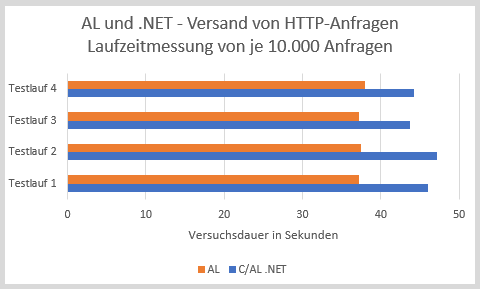
\includegraphics{images/Tests-WS}
	\caption{Grafische Darstellung der Messergebnisse der Laufzeitmessungen}
	\label{fig:Test1Graphical}
\end{figure}

Die Messungen zeigen wie erwartet, dass die in die Sprache integrierte Funktionalität ein leicht besseres Laufzeitverhalten zeigt. Trotz des Mehraufwandes des Ladens einer externen Klassenbibliothek und deren Verwendung, verhält sich die AL-Variante jedoch im Durchschnitt lediglich 16\% performanter.
\pagebreak

\section{Tabellenanpassung und Tabellenerweiterung}
Wie im Unterkapitel Objektarten in Business Central \ref{fig:TableExtension} erwähnt, können in der erweiterungsbasierten Programmierung unter AL zu bestehenden Tabellenobjekten keine neuen Felder direkt hinzugefügt werden. Um  dennoch die Möglichkeit zu wahren, die Standardtabellen zu erweitern, wurde der Objekttyp der Tabellenerweiterung eingeführt. In Objekten vom Typ Erweiterungstabelle platzierte Felder werden in der Datenbank ein einer eigenen Tabelle abgelegt. Diese zusätzliche Tabellen sind unbedingt nötig, um Daten der Erweiterung von denen der Standardapplikation zu kapseln, und so zu garantieren, dass die Standardapplikation ohne manuelle Eingriffe mit Updates versorgt werden kann. Gleichzeitig hat dieses Verhalten jedoch auch zur Folge, dass der Zugriff auf die zusätzlichen Felder mit einer \textit{Join-Operation} erfolgen muss. In weiterer Folge können diese Felder auch nicht als \textit{SumIndexField} in einem Tabellenindex verwendet werden kann. 

Ziel der folgenden Testreihe ist es, den Unterschied zwischen einer traditionell zum Tabellenobjekt hinzugefügten Feld, und einem via Erweiterungsobjekt erstelltem Feld zu quantifizieren. Zu diesem Zweck wird die C/AL Variante der Tabelle \textit{Loyalty Point Entry} \ref{fig:Tables} mittels einer neuen Erweiterung um ein neues Feld \textit{Points2} erweitert, sodass sich folgendes Tabellenschema ergibt:

\begin{figure}[H]
	\centering
	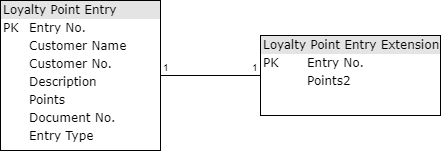
\includegraphics[width=110mm]{images/Test2}
	\caption{Tabellenschema Treuepunktposten und zugehörige Erweiterung}
	\label{fig:Test2Schema}
\end{figure}

\paragraph{}
Um die Abfrage um herauszufinden, wie viele Treuepunkte ein Kunde momentan hat, möglichst effizient gestalten zu können, wird in der C/AL Variante - also dem Feld \textit{Points} ein nach \textit{Customer No.} gruppierter Index erstellt. Da \textit{Points2} sich auf Datenbankseite nicht in der selben Tabelle befindet, lassen sich derartige Zugriffsoptimierungen via Indizes hier nicht verwirklichen. Für den folgenden Test werden für zehn Kundeneinträge je 10.000 Treuepunktposten erstellt. Gemessen wird die Zeit, welche die Microsoft Dynamics 365 Business Central Instanz benötigt, um für jeden der Kunden den Treuepunktsaldo zu ermitteln. In dieser Messreihe wird das Gesamtsystem (Datenbank + Serverinstanz) nach jeder Messung neu gestartet, um Effekte durch Zwischenspeicherungen auszunehmen.

\begin{figure}[H]
	\centering
	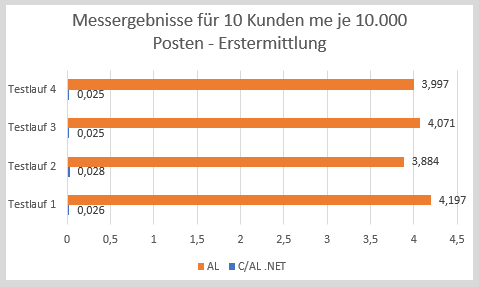
\includegraphics[width=110mm]{images/Test2NoCache}
	\caption{Messung: Aggregierung von Treuepunktposten - Ohne Zwischenspeicher}
	\label{fig:Test2Schema}
\end{figure}

Hier lässt sich ein deutlicher Unterschied in Bezug auf die Berechnungszeiten feststellen. Die Differenz rührt daher, da das via C/AL erstellte Feld auch gleichzeitig von Microsoft Dynamics 365 Business Central als \textit{SumIndexField} angelegt wurde. Anhand der angegebenen \textit{SumIndexFields} kann Microsoft SQL Server materialisierte Sichten erstellen, um Daten bereits beim Einfügen zu aggregieren. Somit wird beim Zugriff auf das Feld in der C/AL Variante keine Summenoperation ausgeführt, sondern lediglich das Ergebnis aus der materialisierten Sicht wiederverwendet, währenddessen muss für die Auswertung des Feldes \textit{Points2} aus dem Erweiterungstabellenobjekt jeder Treuepunktposten mit seinem Äquivalent aus der Erweiterungstabelle verbunden werden, und danach die Summe der einzelnen Werte berechnet werden. Dies würde bedeuten, dass jede Berechnung den Nutzer einige Sekunden an Zeit kosten würde. In dieser Testreihe werden lediglich 10.000 Datensätze verwendet, in einem Produktivszenario sind jedoch oft wesentlich größere Datenquellen vorhanden. Um diese Probleme zu mindern, verwendet Microsoft Dynamics 365 Business Central ein komplexes Zwischenspeichersystem, das oft verwendete Datenbestände im Hauptspeicher verwaltet und vor-aggregiert. 
Vor der folgenden Messung wurde das System nicht durchgestartet. Die Serverapplikation hat hier bereits Treuepunktdaten im Hauptspeicher vorberechnet. Dies ist der Zustand in dem sich das System im Normalzustand befindet.
\begin{figure}[H]
	\centering
	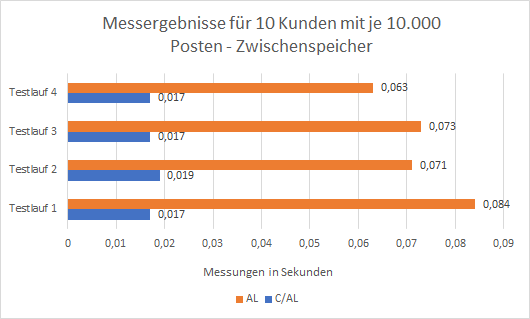
\includegraphics[width=110mm]{images/Test2Cache}
	\caption{Messung: Aggregierung von Treuepunktposten - mit Zwischenspeicher}
	\label{fig:Test2Schema}
\end{figure}

Der Zugriff auf die relevanten Daten dauert in diesem Zustand zwar immer noch etwas vier mal länger, Berechnungszeiten von unter 100 Millisekunden sind jedoch bei Operationen dieser Art durchaus vertretbar.

\section{Codeanpassung und ereignisorientierte Codeerweiterung}
Mit der Einführung der Erweiterungsentwicklung und AL, werden den Entwicklern rund um die Welt viele neue Möglichkeiten präsentiert. Einerseits ändern sich mit dem erweiterungsbasierten Ansatz Lizenz- und Finanzierungsmodelle, andererseits werden dadurch Entwicklern neue Vertriebsmöglichkeiten zugänglich gemacht. Erweiterungen können ohne mitwirken des Entwicklers beim Endkunden, und durch den Endkunden selbst installiert werden, da die Integration einer Erweiterung laut technischer Spezifikation keine manuell auszuführenden Tätigkeiten bedingt.

Andererseits werden Entwickler durch diesen Umschwung jedoch auch technologisch eingeschränkt. Anpassungen des Microsoft-Standard Codebestands waren seit Ersterscheinung des ERP-Systems der einzige und bevorzugte Weg, um Änderungen am Verhalten des Systems vorzunehmen. Diese Codeanpassungen geben dem Entwickler vollständige Kontrolle über den Ablauf der einzelnen Teilprozesse im Gesamtsystem. So können Entwickler Programmcode an beliebigen Stellen hinzufügen, bearbeiten oder auch entfernen.

Mit der Einführung der erweiterungsorientierten Entwicklung sind Codeanpassungen nicht mehr möglich. Standard-Applikationsobjekte können nicht mehr verändert werden, lediglich Erweiterungen sind noch möglich. Dies würde jedoch auch bedeuten, dass Entwickler nicht mehr die Möglichkeiten hätten, im Microsoft Standard abgebildete Prozesse abzuändern. Um Entwicklern dennoch Anpassungen der Standardlogik zu ermöglichen, wird seitens Microsoft ein Mechanismus eingeführt, der in anderen Sprachen und Plattformen seit Jahrzehnten zum Standardumfang zählt: Ereignisse (\textit{Events}).

Seit dem Ersterscheinen von Ereignissen in der Version 2016, werden in der gesamtem Applikation und in sämtlichen Prozesslogiken Ereignisse gefeuert. Entwickler können sich an diese Ereignisse binden und je nachdem welche Ereignisse auftreten, spezielle Logikteile ausführen. Mittlerweile befinden sich in der aktuellen Version von Microsoft Dynamics 365 Business Central mehrere tausend Ereignisse, die aus Codeunit-Applikationsobjekten gefeuert werden.

So erlaubt uns ein Ereignis beispielsweise, darauf zu reagieren, nachdem ein Benutzer beim Drucken eines Berichts einen Drucker auswählt. Das Ereignis hierfür kommt aus dem Codeunit-Applikationsobjekt \textit{ReportManagement}, und mit dem folgenden Codestück kann man auf dieses Ereignis reagieren: 

\begin{program}[H]  % Start your code-block
	\begin{JavaCode}
[EventSubscriber(ObjectType::Codeunit, Codeunit::ReportManagement, 'OnAfterGetPrinterName', '', false, false)]
  local procedure OnGetPrinterName(ReportID: Integer; VAR PrinterName: Text[250])
  begin
    //Place custom code here
  end;
	\end{JavaCode}
\end{program}

Microsoft stellt mit den gefeuerten Ereignissen in der Codebasis tausende Stellen bereit, um sich in die einzelnen Prozessschritte des Gesamtsystems einzuhaken. Zusammenfassend könnte man meinen, dass dadurch die Notwendigkeit von Codeanpassungen vollständig verschwunden wäre. Dem ist jedoch leider nicht so, denn während Ereignisse eine elegante Möglichkeit bieten, Standardvorgehensweisen im System zu manipulieren, hat auch Ereignismechanismus seine Einschränkungen und Schwächen:

\begin{itemize}
	\item Was passiert, wenn mehrere Programmstücke auf das selbe Ereignis reagieren wollen? Konkret geht es darum um die Ausführungsreihenfolge. Welcher der reagierenden Codestücke werden zuerst ausgeführt? Da man als Entwickler davon ausgehen muss, dass eine entwickelte Erweiterung auf fremden System ausgeführt wird, ist diese Frage von hoher Wichtigkeit. Denn wenn mehrere Codestücke dieselben Daten ändern, kann es schnell zu Inkonsistenzen kommen. Und inkonsistente Daten können in der Welt der Finanzbuchhaltung schnell zu rechtlichen Schwierigkeiten führen. Bei Änderung eines Systems via Codeanpassung kommt diese Frage nicht auf, die Ausführungsreihenfolge ist strikt durch den Ablauf des Programmcodes gegeben. Auf die Frage, welches Codestück zuerst ausgeführt wird, gibt es keine klare eindeutige Antwort. Im Optimalfall ist der reagierende Code so zu gestalten, dass er weder durch vorhergehende Ereignisbindungen beeinträchtigt wird, noch darauffolgende Ereignisbindungen beeinträchtigt. In sehr vielen Anwendungsfällen ist dies jedoch schlichtweg nicht möglich.
	\item Die Ereignisarchitektur schränkt Entwickler dramatisch ein. Entwickler können nur noch dort eingreifen, wo ein Eingriff seitens Microsoft auch vorgesehen ist. Und selbst an diesen Punkten kann man Prozesse aus der Basiscode nur beschränkt modifizieren, da man als Entwickler meist keinen Zugriff auf den Zustand aller lokalen und globalen Variablen innerhalb der aufrufenden Funktion hat. Um das vergleichbares Maß an Flexibilität wie Codeanpassungen zu bieten, wäre praktisch nach jeder Zeile Code in der Standardapplikation eine Ereignisauslösung notwendig.
\end{itemize}

\section{Sourcecode Verwaltung und CI/CD}
Mit der Nutzung von Visual Studio Code haben Microsoft Dynamics 365 Business Central Entwickler erstmals in der Geschichte der ERP-Lösung Zugriff auf einen modernen dateibasierten Quellcode-Editor. Programmcode wird nicht mehr primär in einer Entwicklungsdatenbank bearbeitet und gespeichert, sondern befindet sich lokal auf der Maschine des arbeitenden Entwicklers. Was für Entwickler sämtlicher höherer Programmiersprachen bereits seit Anfang der 90er Jahren Standard ist, gilt seit 2018 auch für Business Central Entwickler. Dabei handelt es sich um einen gigantischen Schritt in die richtige Richtung. 

Im Rahmen der \textit{Mibuso NAVTechDays} \footnote{www.mibuso.com} im November 2018 in Antwerpen, der wohl bedeutendsten Entwicklerkonforenz des Jahres für NAV und Business Central Entwickler im europäischen Raum, wurde während eines Vortrags erhoben, wie viele der Anwesenden Entwickler Sourcecode Verwaltungssysteme wie Git für ihre C/AL Projekte verwenden. Die ernüchternde Antwort: nur etwa 10-15\% der Anwesenden Entwickler verwenden für C/AL Programmcode ein entsprechendes Verwaltungssystem. Die Gründe hierfür sind naheliegend: Wenn Programmcode nicht bereits während des Entwicklungsprozesses lokal in Dateiform auf dem Entwicklerrechner vorhanden ist, stellt die Nutzung eines Systems wie Git einen Mehraufwand dar, und verkompliziert den Entwicklungsprozess. Hier ist es oft einfacher und zielführender, nächtlich automatisiert Sicherungen der Entwicklungsdatenbank zu erstellen, und diese bei Bedarf wiederherzustellen.







\chapter{Diskussion}
\label{cha:Diskussion}


%%%----------------------------------------------------------
\MakeBibliography                        % Quellenverzeichnis
%%%----------------------------------------------------------
%%% Messbox zur Druckkontrolle ------------------------------

%%%----------------------------------------------------------
\end{document}
%%%----------------------------------------------------------